
\section{Lake at rest with a steep island}

This is a test if the method is well-balanced. Furthermore, we test if the wet/dry interface has been correctly treated for a steep island. This test is taken from the work of Mungkasi and Roberts~\cite{MR2010}.

The initial condition is a lake at rest with water depth $4.5$. The topography is
\begin{equation}
z(x,y)= \left\{ \begin{array}{ll}
             -0.01(x-200) + 4& ~\textrm{if}\quad 0 \leq x < 200\\
             -0.02(x-200) + 4& ~\textrm{if}\quad 200 \leq x < 300\\
             -0.01(x-300) + 2& ~\textrm{if}\quad 300 \leq x < 400\\
             (-1/75)(x-400) + 2& ~\textrm{if}\quad 400 \leq x < 550\\
             (1/11250)(x-550)(x-550)& ~\textrm{if}\quad 550 \leq x < 700\\
             0.03(x-700)& ~\textrm{if}\quad 700 \leq x < 800\\
             -0.03(x-800) + 3& ~\textrm{if}\quad 800 \leq x < 900\\
             6& ~\textrm{if}\quad 900 \leq x < 1000\\
             (-1.0/20000)(x-1000)(x-1400)& ~\textrm{if}\quad 1000 \leq x < 1400\\
             0& ~\textrm{if}\quad 1400 \leq x < 1500\\
             3& ~\textrm{if}\quad 1500 \leq x < 1700\\
             -0.03(x-1700) + 3& ~\textrm{if}\quad 1700 \leq x < 1800\\
             (4.5/40000)(x-1800)(x-1800) + 2 & ~\textrm{otherwise,}\\
\end{array} \right.
\end{equation} 
The analytical solution is the lake at rest, that is, $w=4.5$ and $u=v=0$.

\subsection{Results}


Current version of \anuga{} might not handle a discontinuous island perfectly. The following three figures show the stage, $x$-momentum, and $x$-velocity respectively, after we run the simulation for some time. We should see excellent agreement between the analytical and numerical solutions if the method is well-balanced and if the wet/dry interface has been correctly treated.

\begin{figure}
\begin{center}
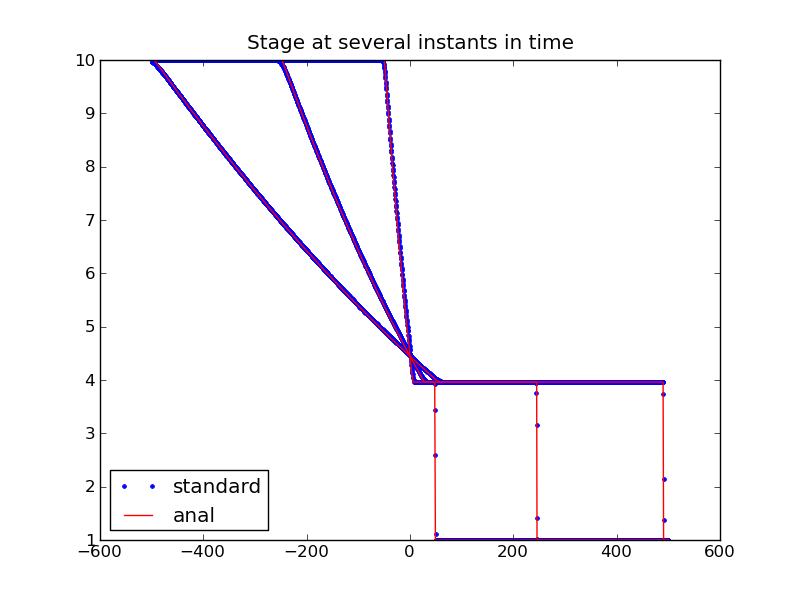
\includegraphics[width=0.9\textwidth]{stage_plot.png}
\end{center}
\caption{Stage results}
\end{figure}


\begin{figure}
\begin{center}
\includegraphics[width=0.9\textwidth]{xmom_plot.png}
\end{center}
\caption{Xmomentum results}
\end{figure}


\begin{figure}
\begin{center}
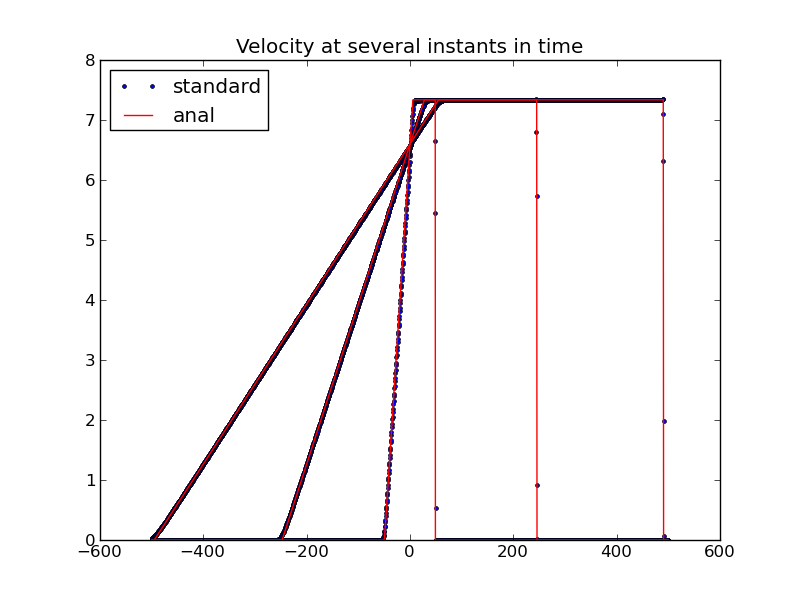
\includegraphics[width=0.9\textwidth]{xvel_plot.png}
\end{center}
\caption{Xvelocity results}
\end{figure}


\endinput
